\begin{frame}
	\frametitle{Moltres}
	\begin{columns}
		\column{5cm}
		Moltres solves the implicitly coupled governing equations for
		neutron diffusion, \gls{DNP} concentrations, and
		temperature.
		
		\vspace{.2cm}
		Moltres requires neutron group constant data, available from any neutron
		transport code (e.g. Serpent, SCALE), for the neutronics calculations.
		
		\vspace{.2cm}
		Moltres accepts various mesh file formats (e.g. exodus, gmsh, etc.)
		\column{5cm}
		\begin{figure}
			\centering
			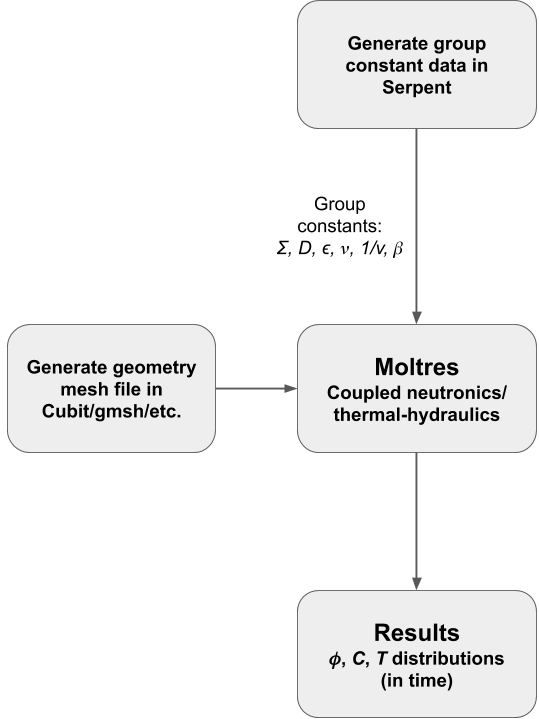
\includegraphics[width=.9\textwidth]{./images/flowchart}
			\caption{Flowchart for running a Moltres simulation.}
			\label{fig:flowchart}
		\end{figure}
	\end{columns}
\end{frame}

\begin{frame}
	\frametitle{Moltres}
	\textbf{Multi-group neutron diffusion}
		\begin{align}
	\frac{1}{v_g} &\frac{\partial \phi_g}{\partial t} - \nabla \cdot D_g \nabla
	\phi_g + \Sigma^r_g \phi_g \nonumber \\ 
	&= \sum^G_{g \neq g'} \Sigma^s_{g' \rightarrow g} \phi_{g'} + \chi^p_g
	\sum^G_{g'=1} (1-\beta) \nu \Sigma^f_{g'} \phi_{g'} + \chi^d_g \sum^I_i
	\lambda_i C_i \label{eq1}
		\end{align}
	\textbf{\gls{DNP} concentration (with advection)}
		\begin{align}
	\frac{\partial C_i}{\partial t} = \sum^G_{g'=1} \beta_i \nu \Sigma^f_{g'}
	\phi_{g'} - \lambda_i C_i
	{\color{red}
	 - \nabla \cdot \overrightarrow{u} C_i}
	\label{eq2}
		\end{align}
		
		Additional advection term in the \gls{DNP} concentration
		equations to account for fuel advection effects.
\end{frame}

\begin{frame}
	\frametitle{Moltres}
		\textbf{Temperature advection-diffusion}
		\begin{align}
	\rho c_{p} \frac{\partial T}{\partial t} + \nabla \cdot \big( \rho
	c_{p} \overrightarrow{u} T - k \nabla T \big) = Q_s - Q_{hx}
	\label{eq3}
		\end{align}
		
		where
		\begin{align*}
		Q_s = \sum^G_{g=1} \epsilon_g \Sigma_g^f \phi_g \label{eq4}
		\end{align*}
		
		Moltres has access to the Navier-Stokes module on \gls{MOOSE} for
		simulating flow. For this work, we assumed plug flow (uniform flow).
\end{frame}

%\begin{frame}
%	\frametitle{Moltres}
%	\textbf{\gls{DNP} drift and decay}
%		\begin{itemize}
%			\item A significant fraction of \gls{DNP} decay outside the active
%			core region
%			\item Moltres 
%		\end{itemize}
%\end{frame}
